\documentclass[a4paper,12pt]{article}

%% Работа с русским языком
\usepackage{cmap}					% поиск в PDF
\usepackage{mathtext} 				% русские буквы в формулах
\usepackage[T2A]{fontenc}			% кодировка
\usepackage[utf8]{inputenc}			% кодировка исходного текста
\usepackage[english,russian]{babel}	% локализация и переносы

%% Отступы между абзацами и в начале абзаца 
\setlength{\parindent}{0pt}
\setlength{\parskip}{\medskipamount}

%% Изменяем размер полей
\usepackage[top=0.5in, bottom=0.75in, left=0.625in, right=0.625in]{geometry}

%% Графика
\usepackage[pdftex]{graphicx}
\graphicspath{{images/}}

%% Различные пакеты для работы с математикой
\usepackage{mathtools}				% Тот же amsmath, только с некоторыми поправками

\usepackage{amssymb}				% Математические символы
\usepackage{amsthm}					% Пакет для написания теорем
\usepackage{amstext}
\usepackage{array}
\usepackage{amsfonts}
\usepackage{icomma}					% "Умная" запятая: $0,2$ --- число, $0, 2$ --- перечисление
\usepackage{bbm}				    % Для красивого (!) \mathbb с  буквами и цифрами
\usepackage{enumitem}               % Для выравнивания itemise (\begin{itemize}[align=left])

% Номера формул
\mathtoolsset{showonlyrefs=true} % Показывать номера только у тех формул, на которые есть \eqref{} в тексте.

% Ссылки
\usepackage[colorlinks=true, urlcolor=blue]{hyperref}

% Шрифты
\usepackage{euscript}	 % Шрифт Евклид
\usepackage{mathrsfs}	 % Красивый матшрифт

% Свои команды\textbf{}
\DeclareMathOperator{\sgn}{\mathop{sgn}}

% Перенос знаков в формулах (по Львовскому)
\newcommand*{\hm}[1]{#1\nobreak\discretionary{}
{\hbox{$\mathsurround=0pt #1$}}{}}

% Графики
\usepackage{tikz}
\usepackage{pgfplots}
%\pgfplotsset{compat=1.12}

% Изменим формат \section и \subsection:
\usepackage{titlesec}
\titleformat{\section}
{\vspace{1cm}\centering\LARGE\bfseries}	% Стиль заголовка
{}										% префикс
{0pt}									% Расстояние между префиксом и заголовком
{} 										% Как отображается префикс
\titleformat{\subsection}				% Аналогично для \subsection
{\Large\bfseries}
{}
{0pt}
{}

% Информация об авторах
\author{Группа лектория ФКН ПМИ 2015-2016 \\
	Анастасия Иовлева \\
	Ксюша Закирова \\
	Руслан Хайдуров}
\title{Лекции по предмету \\
	\textbf{Линейная алгебра и геометрия}}
\date{2016 год}

\newtheorem*{Def}{Определение}
\newtheorem*{Lemma}{Лемма}
\newtheorem*{Suggestion}{Предложение}
\newtheorem*{Examples}{Пример}
\newtheorem*{Comment}{Замечание}
\newtheorem*{Consequence}{Следствие}
\newtheorem*{Theorem}{Теорема}
\newtheorem*{Statement}{Утверждение}
\newtheorem*{Task}{Упражнение}
\newtheorem*{Designation}{Обозначение}
\newtheorem*{Generalization}{Обобщение}
\newtheorem*{Thedream}{Предел мечтаний}
\newtheorem*{Properties}{Свойства}

\renewcommand{\mathbb}{\mathbbm}
\renewcommand{\Re}{\mathrm{Re\:}}
\renewcommand{\Im}{\mathrm{Im\:}}
\newcommand{\Arg}{\mathrm{Arg\:}}
\renewcommand{\arg}{\mathrm{arg\:}}
\newcommand{\Mat}{\mathrm{Mat}}
\newcommand{\id}{\mathrm{id}}
\newcommand{\isom}{\xrightarrow{\sim}} 
\newcommand{\leftisom}{\xleftarrow{\sim}}
\newcommand{\Hom}{\mathrm{Hom}}
\newcommand{\Ker}{\mathrm{Ker}\:}
\newcommand{\rk}{\mathrm{rk}\:}
\newcommand{\diag}{\mathrm{diag}}
\newcommand{\ort}{\mathrm{ort}}
\newcommand{\pr}{\mathrm{pr}}
\newcommand{\vol}{\mathrm{vol\:}}

\renewcommand{\epsilon}{\varepsilon}
\renewcommand{\phi}{\varphi}
\newcommand{\e}{\mathbb{e}}
\renewcommand{\l}{\lambda}
\renewcommand{\C}{\mathbb{C}}
\newcommand{\R}{\mathbb{R}}
\newcommand{\E}{\mathbb{E}}

\newcommand{\vvector}[1]{\begin{pmatrix}{#1}_1 \\\vdots\\{#1}_n\end{pmatrix}}
\renewcommand{\vector}[1]{({#1}_1, \ldots, {#1}_n)}

\begin{document}

\section*{Лекция 9 от 9.02.2016}

\subsection{Продажа земли}

Предположим, что у нас есть участок земли у берега и мы хотим его продать.
При этом у нас есть несколько покупателей и каждый из них готов отдать некоторую сумму за некоторый фрагмент участка.
Как максимизировать выгоду?

Формализуем: у нас есть $n$ предложений и каждое характеризуется тремя числами — началом $s$, концом $f$ и весом $w$.
Таким образом, вход выглядит так:

$s_1, \ldots, s_n$ --- начала

$f_1, \ldots, f_n$ --- концы

$w_1, \ldots, w_n$ --- веса\\

Пример:

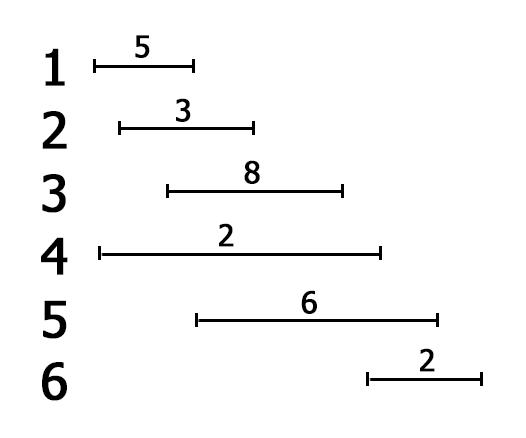
\includegraphics[width=5cm]{09_intervals.png}\\

На выходе мы хотим получить максимальную сумму весов непересекающихся интервалов:

\[
\max\limits_{T\subseteq \left\{ 1,\ldots, n \right\}} \sum\limits_{i\in T}w_i 
\]
\[
T: \forall i<j \implies f_i \leqslant s_j \lor f_j \leqslant s_i
\]

Перебором задача решается за $O(2^n)$

Давайте в качестве первого шага отсортируем по правым концам за $O(n\log n)$.

Введём обозначения:

O --- оптимальное решение

$OPT(i)$ — максимальаня стоимость оптимального решения для первых $i$ интервалов

$OPT(n)$ — Максимальная стоимость оптимального решения длв всех интервалов\\

Пример:

\[
    \mathrm{OPT}(6) = \max\begin{cases}
        \mathrm{OPT}(5), 6\not\in O;\\
        2+ \mathrm{OPT}(3), 6\not\in O; \text{(так как все до третьего не пересекаются с шестым)}
    \end{cases}
\]

Пусть $p(j) = \max\left\{ i<j \mid f_{i}\leqslant s_j\right\}$ --- первый интервал до $j$-го, совместимый с ним (то есть не пересекающийся).

Эффективное вычисление $p$ остается в качестве упражнения.

Тогда общая формула для $OPT$ такова:
\[
    \mathrm{OPT}(i) = \max\begin{cases}
        \mathrm{OPT}(i-1);\\
        w_i+ \mathrm{OPT}(p(i));
    \end{cases}
\]


\begin{algorithm}
	\caption{Подсчёт $OPT(i)$}
	\begin{algorithmic}[1]
		\Function{ComputeOpt}{i}
			\If{\(i = 0\)}
				\State return 0
			\EndIf
			\State return \(\max \{\textsc{ComputeOpt}(i - 1), w_i + \textsc{ComputeOpt}(p(i))\}\)
		\EndFunction
	\end{algorithmic}
\end{algorithm}

Считая, что данные уже отсортированы, получим что сложность равна $O(n)$, но только если мы сохраняем результаты вычислений.
Иначе мы делаем много лишних вычислений, и время будет таким: $T(n) = T(n-1)+T(n-2)+c$.
Очень похоже на числа Фибоначчи, а они растут экспоненциально; это выражение --- тоже.


Значит надо сохранять вычисления в некоторый массив OPT.
Инициализируем его так: 
\[
\mathrm{OPT} = [0, -1, \ldots, -1]
\]

\begin{algorithm}
	\caption{Модифицированный подсчёт $OPT(i)$}
	\begin{algorithmic}[1]
		\Function{ComputeOpt}{i}
			\If{\(OPT(I) < 0\)}
				\State \(OPT[i] = \max \{\textsc{ComputeOpt}(i - 1), w_i + \textsc{ComputeOpt}(p(i))\}\)
			\EndIf
			\State return \(OPT[i]\)
		\EndFunction
	\end{algorithmic}
\end{algorithm}

Вот теперь сложность алгоритма --- $O(n)$

Так как мы вычисляем 1 раз каждый элемент $OPT$, мы можем избавиться от рекурсии:\\

\begin{algorithm}
	\caption{Модифицированный подсчёт $OPT(i)$ без рекурсии}
	\begin{algorithmic}[1]
		\Function{ComputeOpt}{i}
			\State $OPT = [0, -1, \ldots, -1]$
			\For{\(OPT(I) < 0\) \textbf{to} \(n\)}
				\State \(OPT[i] = \max \{OPT[i - 1], w_i + OPT[p(i)]\}\)
			\EndFor
			\State return \(OPT[n]\)
		\EndFunction
	\end{algorithmic}
\end{algorithm}

Как теперь определить, какие именно участки нужно продать?
Можно хранить в $OPT$ на $i$-ом месте необходимые участки, но это замедлит нашу программу (не асимптотически), так как придётся тратить на запись не константное время, а некоторое $O(n)$.
Однако, можно восстановить номера участков по массиву $OPT$:

\begin{algorithm}
	\caption{Восстановление решения}
	\begin{algorithmic}
		\Function{FindSolution}{OPT}
			\State \(T = \emptyset\)
			\State \(i = n\)
			\While{\(i > 0\)}
				\If{\(OPT[i - 1] > w_i + OPT[p(i)]\)}
					\State \(i = i - 1\)
				\Else
					\State \(T = T \cup {i}\)
					\State \(i = p(i)\)
				\EndIf
			\EndWhile
			\State return \(p(i)\)
		\EndFunction
	\end{algorithmic}
\end{algorithm}

\subsection{В общем о динамическом программировании}
Чем оно отличается от ``Разделяй и властвуй''? А тем, что задачи могут пересекаться. Ведь при использовании классического ``разделяй и властвуй'' мы бы получили экспоненциальное решение. 

Для эффективного использования этого принципа необходимы следующие условия:
\begin{itemize}
    \item Небольшое число задач; например, полиномиальное;
    \item Возможность их упорядочить и выразить решения следующих через предыдущие.
\end{itemize}

\subsection{Задача с прошлой лекции --- выравнивание текста}

Дано:\\
$w_1,\ldots, w_n$ --- длины слов.

$c(i, j)$ --- штраф за размещение $w_i,\ldots, w_j$ на одной строке.\\

Преобразуем наше рекурсивное решение в итеративное.

OPT$(i)$ --- оптимальное размещение $w_i, \ldots, w_n$.

OPT(i) = $\min\limits_{i\leqslant j\leqslant n} \left\{ c(i, j)+ \mathrm{OPT}(j+1) \right)\}$.\\

Запишем итеративный алгоритм для этой формулы.
Так как $i$-ая задача зависит от задач с большим индексом, будем заполнять массив с конца.

\begin{algorithm}
	\caption{Выравнивание текста}
	\begin{algorithmic}
		\Function{ComputeOpt}{$w_1, \ldots, w_n$}
			\State \(best = [0] \times n\)
			\State \(OPT = [+\infty] \times (n + 1)\)
			\State $OPT[n + 1] = 0$
			\For{\(i \mathrel{:=} n\) \textbf{downto} 1}
				\For{\(j \mathrel{:=} i\) \textbf{to} n}
					\If{\(c(i, j) + OPT[j + i] \leqslant OPT[i]\)}
						\State \(OPT[i] = c(i, j) + OPT[j + i]\)
						\State \(best[i] = j\)
					\EndIf
				\EndFor
			\EndFor
			\State return $OPT[i]$
		\EndFunction
	\end{algorithmic}
\end{algorithm}

Как видно, в данном алгоритме решение строится по ходу, потому что в данном случае это допустимо.

\end{document}
